\documentclass[10pt]{article}
\usepackage[letterpaper,top=1in,bottom=1in,left=1in,right=1in,headsep=14pt]{geometry}
\usepackage[T1]{fontenc}
\usepackage[utf8]{inputenc}
\usepackage{XCharter}
\usepackage[xcharter,vvarbb]{newtxmath}
\usepackage[scaled=0.96]{sourcesanspro}
\usepackage{microtype}
\usepackage{amsmath}
\usepackage{graphicx}
\usepackage{booktabs}
\usepackage{longtable}
\usepackage{array}
\usepackage{float}
\usepackage{xcolor}
\usepackage[font=small,labelfont=bf,skip=6pt]{caption}
\usepackage{fancyhdr}
\usepackage[section]{placeins}
\usepackage[numbers,sort&compress]{natbib}
\usepackage[colorlinks=true,linkcolor=ink,citecolor=accent,urlcolor=accent]{hyperref}
\usepackage{xurl}
\newcolumntype{L}[1]{>{\raggedright\arraybackslash}p{#1}}
\graphicspath{{figs/}}

\definecolor{accent}{HTML}{8A1C1C}
\definecolor{ink}{HTML}{1A1A1A}
\definecolor{grey}{HTML}{6B6B6B}
\definecolor{rule}{HTML}{C8C8C8}

\newcommand{\lmes}{LongMemEval-S}
\newcommand{\nany}[1]{NDCG$_{\mathrm{any}}$@#1}
\newcommand{\rall}[1]{Recall$_{\mathrm{all}}$@#1}
\newcommand{\pub}{$^{\dagger}$}
\newcommand{\tun}{$^{\ddagger}$}
\newcommand{\ours}[1]{\textbf{#1}}
\newcommand{\pending}[1]{\colorbox{yellow!40}{\texttt{#1}}}
\newcommand{\hairline}{\par\noindent{\color{rule}\rule{\textwidth}{0.4pt}}\par}
\setlength{\emergencystretch}{2em}
\renewcommand{\topfraction}{0.9}
\renewcommand{\bottomfraction}{0.6}
\renewcommand{\textfraction}{0.07}
\renewcommand{\floatpagefraction}{0.45}
\setcounter{topnumber}{3}
\setcounter{totalnumber}{4}
\setlength{\columnwidth}{\textwidth}
\makeatletter
\setlength{\@fptop}{0pt}
\setlength{\@fpsep}{2.2em}
\setlength{\@fpbot}{0pt plus 1fil}
\makeatother
\clubpenalty=10000
\widowpenalty=10000
\displaywidowpenalty=10000

\pagestyle{fancy}
\fancyhf{}
\renewcommand{\headrulewidth}{0pt}
\fancyhead[L]{\sffamily\footnotesize\color{grey}Memorable: Compact Verbatim Memory for Long Conversations}
\fancyhead[R]{\sffamily\footnotesize\color{grey}\thepage}
\fancypagestyle{plain}{\fancyhf{}\renewcommand{\headrulewidth}{0pt}\fancyfoot[C]{\footnotesize\color{grey}\thepage}}

\renewenvironment{abstract}
  {\vspace{1.2em}\hairline\vspace{0.9em}\noindent{\large\bfseries Abstract}\par\vspace{0.45em}\noindent\ignorespaces}
  {\par\vspace{1.1em}\hairline\vspace{0.4em}}

\begin{document}
\thispagestyle{plain}
\begin{flushright}\sffamily\small\color{grey}November 9, 2026\end{flushright}
\hairline
\vspace{14pt}
{\noindent\fontsize{24}{29}\selectfont\bfseries\color{ink} Memorable: Compact Verbatim\\Memory for Long Conversations\par}
\vspace{12pt}
{\noindent\large Nikhil Krishnaswamy$^{1,2}$, Advaiyt Sane$^{2,3}$\par}
\vspace{4pt}
{\noindent\sffamily\footnotesize\color{grey}$^{1}$Stanford University, USA; $^{2}$Memorable, San Francisco, USA; $^{3}$Carnegie Mellon University, USA\par}
\vspace{8pt}
{\noindent\sffamily\footnotesize\textbf{Correspondence}\hspace{0.45em}\href{mailto:nikhil@memorable.sh}{nikhil@memorable.sh}, \href{mailto:advaiyt@memorable.sh}{advaiyt@memorable.sh}\par}
{\noindent\sffamily\footnotesize\textbf{Code, results and registered predictions}\hspace{0.45em}\href{https://github.com/MemorableOrg/compact-verbatim-memory}{github.com/MemorableOrg/compact-verbatim-memory}\par}
\vspace{10pt}
\hairline
\vspace{10pt}
\begin{abstract}
Agent memory systems often ask a language model to decide what to remember before future questions are known. This adds ingestion cost and can discard details that later matter. We investigate whether effective memory requires this generative write step. Our approach preserves the original history and retrieves evidence when a question arrives, with no generative model calls to construct the store: conversation turns, or whole agent trajectories, are kept as they were, indexed by keyword and by a local embedding model, and reordered at question time by a fused score, two dialogue rules and two local cross-encoders. An agent pays a memory's build and read costs on every session while a benchmark score is paid once, so we report accuracy together with tokens read, search time and build cost. With GPT-5 reading the top 40 stored turns, the store answers 90.6 percent of 607 LoCoMo questions, 385 of them development questions used to tune the search, and 82.0 percent of the 222 test questions completed, at 3,294 reader tokens per question and about one second of search. Retrieval holds up without model-written memories: the store finds every gold session in the top 10 for 97.4 percent of 470 LongMemEval-S questions, including development questions used for tuning, recovers 80.3 percent of LoCoMo gold turns in the top 10 against 64.0 for a flat retrieval baseline, and ranks agent trajectories on Proced-Mem at 0.957 mean average precision. The remaining errors expose a tradeoff between preserving information and finding all the evidence needed to answer. These results motivate agent memory that retains the evidence and leaves its interpretation to the moment of use. The code, the per-question results and the protocol that registered every run are public.
\end{abstract}

\section{Introduction}
\label{sec:intro}

We propose an agent memory without a generative writer. Here, a writer is a language model that selects and rewrites past interactions for storage. Our approach retains the original history and retrieves relevant evidence when a question arrives. Agent memories make information from earlier interactions available to later tasks \citep{packer2023memgpt,park2023generative}. Many use a generative model to construct the stored representation. Mem0 extracts and updates facts \citep{chhikara2025mem0}, Zep constructs a temporal knowledge graph \citep{rasmussen2025zep}, and Letta's agents edit memory files \citep{letta2025sleeptime,packer2023memgpt}. Workflow memories similarly use a model to derive guidance from past agent runs \citep{fang2026memp,ouyang2026reasoningbank,wang2025agent}.

Generative writing introduces three possible costs. First, extraction and update calls add ingestion cost as the history grows, even when no later question uses the stored information \citep{chhikara2025mem0,rasmussen2025zep}. Second, sampling can produce different stores from the same history, so reproducing a memory requires more than its construction code. Third, the writer can omit or alter details that later questions need. One audit of a Mem0 deployment classified 97.8 percent of 10,134 stored entries as junk \citep{mem0issue4573}; this is evidence from one deployment rather than a general failure rate. An agent that runs across thousands of sessions pays these costs on every one of them, while a benchmark score is paid for once, so we treat a memory result as a claim about accuracy together with tokens read, search time and build cost. We investigate what can be achieved without generative write calls. Our main LoCoMo comparison uses Mem0's published reader, judge and prompts on both sides.

Our memory stores each conversation turn verbatim, together with its speaker and date (Figure~\ref{fig:method}). To retrieve relevant evidence, we combine a keyword search for matching words with an embedding search for similarity in meaning. On LoCoMo, this produces an initial ranking of turns that we refine in three further stages. A dialogue rule passes part of each turn's score to the next turn in the same session, helping surface replies that do not repeat the question's words. A second rule boosts turns spoken by the person the question is about. Two local models, called cross-encoders, then rescore the leading candidates by evaluating each turn together with the question. A reader language model answers from the highest-ranked original turns, presented in chronological order. On LongMemEval-S, the keyword and embedding searches rank whole sessions without these later stages. We also adapt this retrieval approach to rank past agent trajectories on Proced-Mem \citep{procedmem}.

The answer comparison on LoCoMo has similar aggregate accuracy under a shared reader, judge and prompts from Mem0's published evaluation \citep{mem0benchmarks2026}. On the 607 questions both systems have answered, our store scores 90.6 against 90.3 while reading 3,294 tokens per question against 6,956, with no generative write calls. This aggregate includes 385 development questions used to tune the search. On the 222 test questions alone, our store scores 82.0 against 85.6. The full test split was not completed, so the aggregate result does not establish parity on unseen questions.

Retrieval can also be measured without a reader. Our store finds every gold session in the top 10 for 97.4 percent of 470 LongMemEval-S questions; EdgeMem and MemGAS report 93.8 and 94.5, respectively \citep{cui2026edgemem,xu2025memgas}. Our result includes scored questions from the 150-question development split used for tuning, and the comparison interprets the published retrieval metric as all-gold recall. On LoCoMo, the store retrieves 80.3 percent of gold turns in the top 10, against 64.0 for a flat fusion of the same two signals.

The error analysis identifies different weaknesses: model-written facts can lose detail on single-hop questions, while retrieval can omit a turn needed for a multi-hop answer. Two search changes motivated by these errors raise test all-gold recall from 90.2 to 94.4 at 150 turns. This measures the share of questions whose gold turns are all retrieved; no reader has been evaluated on the changed ranking. On Proced-Mem, the retriever reaches 0.957 mean average precision against the benchmark's 0.796. That retriever was selected on the same 40 queries used to score it.

Every main comparison in the paper is in Table~\ref{tab:headline} with its interval, and Figure~\ref{fig:beat} draws the main ones, so that a reader can see at once where the store beats, ties and loses. We mark the rows where tuning touched the scored questions, we state the judge on every row, and we claim a lead only where the difference lies outside its interval under a shared setup. Every run was registered with a prediction before it started, each miss is reported, and the runs that the model budget stopped are reported on the questions they finished and listed with their predictions in Section~\ref{sec:pending}.

Six terms recur. The reader is the language model that answers from the retrieved text, and the judge is the language model that marks an answer right or wrong. A gold turn is a turn the benchmark marks as evidence for the answer, and all-gold recall at $k$ is the share of questions whose gold turns are all among the top $k$ retrieved. A tuned mark (\tun{}) flags a row that includes questions the system was tuned on. A band is a comparison whose two sides were judged by different models; it places a system near another and does not rank them.

\begin{table*}[t]
\caption{Every main comparison in one place. Beats and loses mean the difference lies outside its 95\% interval or margin. Tie means it does not. Band means the two rows differ in judge and cannot be ranked. \tun{} marks a row that includes questions the system was tuned on. One judge means both systems' existing answers were re-scored by Claude Sonnet 5.5 under the same prompt. Section~\ref{sec:setup} gives the interval methods and the caveats on the published rows.}
\label{tab:headline}
\footnotesize
\centering
\setlength{\tabcolsep}{3.5pt}
\begin{tabular}{@{}L{40mm}rL{27mm}L{27mm}L{24mm}L{22mm}@{}}
\toprule
Benchmark and measure & Ours & Comparator & Difference & Setup & Verdict \\
\midrule
LongMemEval-S, all gold sessions in top 10, 470 q.\tun{} & 97.4 & EdgeMem 93.8 & +3.6, margin 2.6 & no reader; published metric inferred & beats \\
LongMemEval-S, all gold sessions in top 3, 470 q.\tun{} & 84.0 & EdgeMem 81.5 & +2.6, margin 4.8 & no reader; published metric inferred & tie \\
LoCoMo, share of gold turns in top 10, 1,152 test q. & 80.3 & flat fusion 64.0, our own baseline & +16.3 [+13.8, +19.2] & no reader & beats \\
Proced-Mem, MAP, 40 queries\tun{} & 0.957 & MiniLM baseline 0.796 & +0.16; judge moves a ranking by up to 0.08 & same judge; no held-out split & beats \\
LoCoMo single-hop accuracy, 256 shared q.\tun{} & 95.7 & Mem0 90.6 & +5.1 [+2.6, +9.2]; the 56 test q. alone +7.1 [$-$1.8, +16.1] & same reader, judge, prompts & beats; tie on test alone \\
LoCoMo accuracy, 607 shared q.\tun{}; tokens 3,294 vs 6,956 & 90.6 & Mem0 90.3 & +0.3 [$-$3.6, +3.6] & same reader, judge, prompts & tie \\
LoCoMo accuracy, the 222 test q. both answered & 82.0 & Mem0 85.6 & $-$3.6 [$-$7.1, $-$0.5] & same reader, judge, prompts & loses \\
LoCoMo accuracy, 607 shared q.\tun{}, one judge & 90.1 & Mem0 90.0 & +0.2 [$-$4.6, +3.5] & same reader and prompts; Claude Sonnet 5.5 judges both & tie \\
LoCoMo accuracy, the 222 test q., one judge & 80.6 & Mem0 85.6 & $-$5.0 [$-$8.1, $-$1.4] & same reader and prompts; Claude Sonnet 5.5 judges both & loses \\
LoCoMo multi-hop accuracy, 130 shared q.\tun{} & 88.5 & Mem0 94.6 & $-$6.2 [$-$11.3, $-$2.5] & same reader, judge, prompts & loses \\
LongMemEval-S accuracy, 319 test q.\tun{}; tokens 19,125 vs 6,787 & 94.0 & Mem0 93.4 on 500 & +0.6 & same reader & band \\
BEAM 1M pass rate, 652 q. & 71.8 & Mem0 70.1 on 700 & +1.7 & same reader & band \\
BEAM 1M pass rate, 652 q., one judge & 61.3 & Mem0 63.9 on 700 & $-$2.6; intervals [57.6, 65.0] and [60.2, 67.3] & same reader; Claude Sonnet 5.5 judges both & tie \\
LoCoMo search time per question, seconds & 1.05 & Mem0 current 3.57, hosted mean; Mem0 2025 paper 0.200, own hardware & $-$2.52 s; +0.85 s & our laptop median; no shared hardware & beats the hosted mean; loses to the 2025 row \\
LoCoMo accuracy, best published row, any reader\tun{} & 90.6 & Zep 94.7, gpt-5.4, third party & $-$4.1 & different reader and judge & band \\
LongMemEval-S accuracy, best published row, any reader & 94.0 & Mastra 94.9, gpt-5-mini & $-$0.9 & different reader and judge & band \\
\bottomrule
\end{tabular}
\end{table*}

\begin{figure*}[t]
\centering
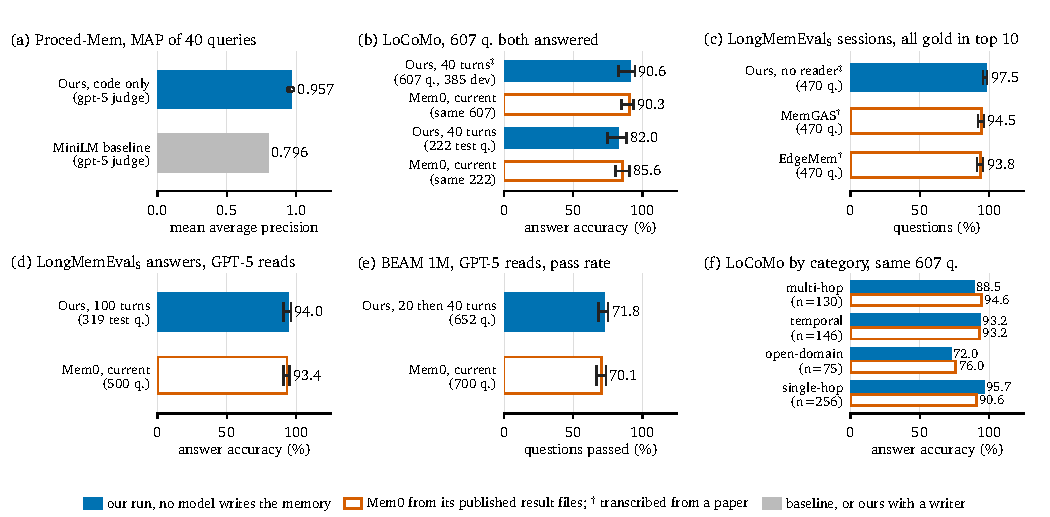
\includegraphics[width=\textwidth]{fig_beat.pdf}
\caption{The main comparisons. Filled bars are our runs. Hollow bars are other systems, read from their published per-question result files unless marked \pub{} (transcribed from a paper). Whiskers are 95\% intervals: conversation-cluster bootstrap in (b), Wilson score intervals for counts out of $n$ elsewhere. (b) and (f) use the 607 LoCoMo questions that both our GPT-5 run and Mem0's file have answered, with Mem0's answer and judge prompts and GPT-5 as reader and judge on both sides; 385 of the 607 are development questions on which the search weights were set (\tun{}), and the lower pair in (b) is the 222 test questions alone. (c) is retrieval with no reader, read as \rall{10}. (d) Our row uses the official LongMemEval judge; Mem0's row uses GPT-5 with its own judge prompt. (e) Our row uses BEAM's judge on gpt-4.1-mini; Mem0's uses GPT-5 with its own prompt. Dots in (a) are the three judge passes.}
\label{fig:beat}
\end{figure*}

\section{Memorable}
\label{sec:method}

A conversation is a sequence of turns $T = (t_1, \dots, t_n)$, each with a speaker, a date and its text $x_i$. Memorable stores $T$ once with fixed code and a local embedder. Its model calls happen at question time (Figure~\ref{fig:method}): a small planner that proposes search queries for the question $q$ and a frozen reader that receives $k$ turns in conversation order and answers. Everything between the two is fixed code, a 33M-parameter embedder and a 278M-parameter cross-encoder, all run on a laptop CPU.

\begin{figure}[t]
\centering
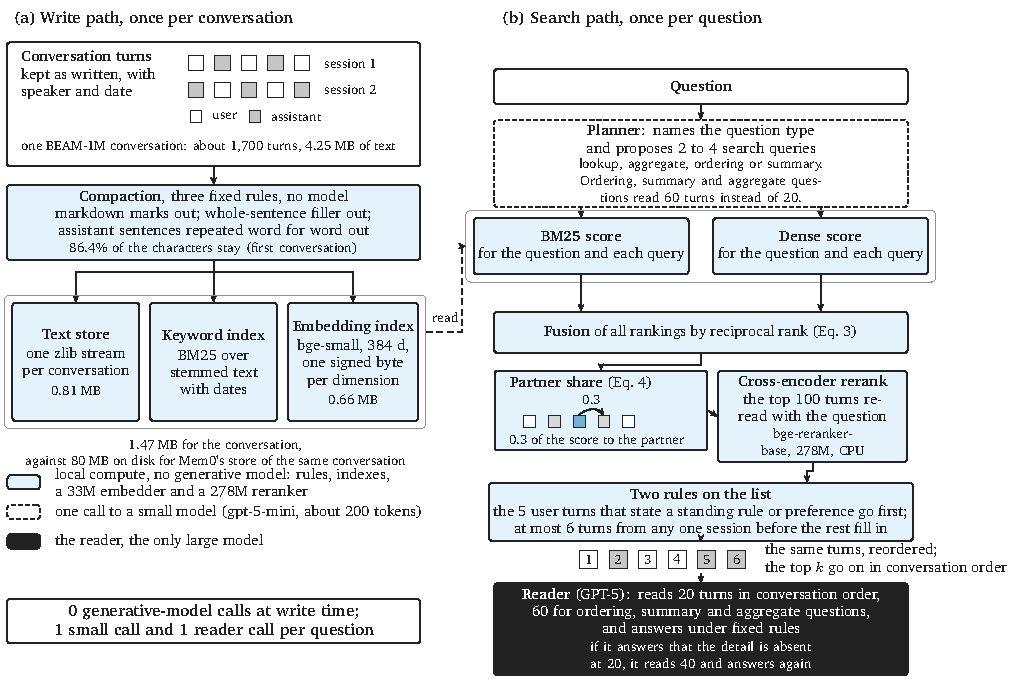
\includegraphics[width=\textwidth]{fig_method.pdf}
\caption{Memorable. (a) The write path runs once per conversation on fixed code and a local embedder. Turns are compacted by three rules, the text is stored with zlib and each turn's embedding as 8-bit integers. (b) The search path runs once per question. A planner proposes two to four queries; keyword and embedding rankings are fused; each turn lends a share of its score to its partner; a cross-encoder rescores the top 100; standing instructions are placed first; at most six turns come from one session; the reader answers from 20 or 60 turns.}
\label{fig:method}
\end{figure}

\subsection{Store}
\label{sec:store}

\paragraph{Compaction.} Assistant prose in a long conversation carries a great deal of markdown decoration, pleasantries and caveats repeated hundreds of times, and each of them costs reader tokens when its turn is retrieved. We remove them with three deterministic maps applied to every turn, $C = R \circ F \circ M$. $M$ strips markdown decoration (heading marks, emphasis stars, horizontal rules, table separator rows and code-fence lines) and replaces table pipes with a spaced bar so that cell contents stay readable. $F$ removes a sentence from either speaker when the whole sentence is a pleasantry or a sign-off, such as ``Certainly!'' or ``Let me know if you need further assistance!''. $R$ removes an assistant sentence longer than 40 characters whose lower-cased, punctuation-stripped form already appeared earlier in the conversation, keeping the first copy. All three maps are string operations. On the first BEAM-1M conversation (1,710 turns, 4.25M characters) the three maps keep 93.1\%, 91.2\% and 86.4\% of the characters in turn, and over all 35 conversations 83\% remain (Figure~\ref{fig:waterfall}). On the 500K development set compaction moved the pass rate by less than two points while cutting the tokens sent to the reader from 23.7K to 19.2K per question.

\paragraph{Storage.} The compacted turns, with their ids, speakers, session indices and dates, are written as one zlib stream per conversation; the session index adds 363 bytes per 1M conversation on average. Each turn's first 256 tokens are embedded once with bge-small-en-v1.5 \citep{xiao2023cpack}, $d = 384$, the vector is unit-normalised, and one signed byte is stored per dimension,
\begin{equation}
\mathbf{q}_i = \mathrm{round}(127\,\mathbf{e}_i), \qquad \hat{s}_i = \mathbf{e}_q^{\top}\mathbf{q}_i / 127 ,
\label{eq:quant}
\end{equation}
so that 384 bytes replace 1,536. The score error is at most $|s_i - \hat{s}_i| \le \|\mathbf{e}_q\|_1 / 254 \le \sqrt{d}/254 \approx 0.077$. We can afford this because the cross-encoder of Section~\ref{sec:search} rescores the top 100 candidates from their text, so the error affects which turns reach that list and leaves their order within it to the cross-encoder; Appendix~\ref{app:int8} compares recall with float and 8-bit vectors. The bytes stored for one conversation are
\begin{equation}
B(T) = |\mathrm{zlib}(C(T))| + n\,d .
\label{eq:bytes}
\end{equation}
Over the 35 BEAM-1M conversations, 159.8~MB of text and 114.6~MB of float vectors become 33.5~MB and 28.7~MB: 62.1~MB stored against 274.4~MB raw, or 1.77~MB per conversation. A stemmed BM25 index over the compacted text \citep{robertson2009bm25}, with each turn's date in its document, is rebuilt from the stored text when a conversation is loaded, so it is left out of $B(T)$.

\subsection{Search}
\label{sec:search}

\paragraph{Planner.} Which turns answer a question depends on its type. A lookup needs the one turn that states a fact, whereas an aggregate, an ordering or a summary needs evidence from many sessions, and a single query rarely reaches them all (Section~\ref{sec:beam}). One call to a small model (gpt-5-mini, about 200 input tokens, about \$0.001 per question) therefore labels the question as a lookup, an aggregate, an ordering (``order'' in the prompt) or a summary and proposes $m \le 4$ search queries $q_1, \dots, q_m$ that together cover it. A question about the days, weeks or months between two events is labelled a lookup, so the reader receives 20 turns; aggregates receive 60.

\paragraph{Fusion.} We rank the turns for the question and for each planner query twice, by BM25 and by embedding cosine, so that a turn can be found by its words or by its meaning. When a turn's date matches a date named in the question, half of the highest BM25 score in that list is added to the turn's BM25 score, which pulls the turns of a named day to the front. Each list is cut to its top 200 and all $2(m+1)$ lists are fused by reciprocal rank \citep{cormack2009rrf},
\begin{equation}
s_i = \sum_{\ell} \frac{1}{60 + r_\ell(i)} ,
\label{eq:rrf}
\end{equation}
where $r_\ell(i)$ is the rank of turn $i$ in list $\ell$. Each turn then lends 0.3 of its score to its neighbour $p(i)$, the other turn of its user-assistant exchange,
\begin{equation}
s'_i = s_i + 0.3\, s_{p(i)} ,
\label{eq:pair}
\end{equation}
because the question often matches one half of the exchange while the answer sits in the other. A local cross-encoder, bge-reranker-base \citep{chen2024bgem3}, reads the question beside the first 1,500 characters of each of the 100 turns with the highest $s'$ and scores how well the turn answers it. The cross-encoder ranking is fused with the earlier ranking by Equation~\ref{eq:rrf} once more, and the 100 candidates stay above every other turn.

\paragraph{Standing rules and a session cap.} Two rules act on the fused list before the reader sees it. The first keeps the user's standing instructions in view. User turns that open with ``always'' or ``never'', or whose first 400 characters contain ``from now on'', ``I prefer'' or ``my preference'', form a pool of standing rules, and the five closest to the question by embedding are placed first, so a rule stated early in the conversation reaches the reader on every later question. The second spreads the read set across sessions: turns are taken from the top of the list, a turn is skipped once six turns from its session have been taken, and the skipped turns fill whatever places remain. The reader receives the first $k = 20$ turns in conversation order, or $k = 60$ for ordering, summary and aggregate questions. If a reader given 20 turns answers that the detail is absent, it is given 40 turns and answers again.

\subsection{Reader}
\label{sec:reader}
The reader (GPT-5) sees each turn, cut to 6,000 characters, with its date and speaker, and answers under fixed rules (Appendix~\ref{app:rules}). The rules about evidence tell it to use only the excerpts, to keep exact names, numbers and dates, to follow standing instructions, and to say that the conversation lacks a detail rather than fill one in. The rules about answers cover the cases a verbatim memory raises that a model-written one has already resolved. The reader prefers the most recent of two conflicting excerpts and says that the fact changed, lists instances with their dates before giving a count, merges repeated mentions of one event, and gives only the most recent value when the question asks for the current one. Four more rules of the same kind, on repeated instructions, relative dates, summaries and the time between two events, are in the full text.

\subsection{Cost}
\label{sec:costmodel}
A memory that a model writes costs $c_w$ per exchange, $N$ in all, and $c_r$ per question, $Q$ in all. Memorable has a write cost of zero and costs $c_p + c_r'$ per question, with $c_p$ the planner call and $c_r'$ the reader:
\begin{equation}
\mathrm{Cost}_{\text{writer}}(Q) = N c_w + Q c_r, \qquad \mathrm{Cost}_{\text{ours}}(Q) = Q\,(c_p + c_r'), \qquad Q^{*} = \frac{N c_w}{c_p + c_r' - c_r} .
\label{eq:cost}
\end{equation}
With the measured values of Section~\ref{sec:cost}, $N c_w = \$7.50$ and $c_p + c_r' = \$0.047$, and an estimated $c_r = \$0.0307$ for Mem0's 200 retrieved facts, the break-even is $Q^{*} \approx 460$ questions per conversation (Figure~\ref{fig:breakeven}). Below it Memorable is cheaper in total; above it Mem0 is, because its reader sees fewer tokens per question. Storage is outside the equation and favours Memorable at every $Q$.

\section{Experiments}
\label{sec:setup}

\paragraph{BEAM.} BEAM has conversations of 100K to 10M tokens, each with 20 questions spread over ten abilities \citep{beam2026}. Our main tier is 1M: 35 conversations and 700 questions, 70 per ability. We chose the settings of Section~\ref{sec:method} on 200-question development sets from the 100K and 500K tiers and registered a prediction before each run. The abilities we chose to target came from an earlier 1M comparison of an earlier version of Memorable, so the 1M tier informed the design. Mem0's answers come from the per-question file it published for its hosted Platform v3 pipeline, a run dated 2026-03-26 with GPT-5 reading its top 200 memories \citep{mem0benchmarks2026}. It is the only per-question BEAM file Mem0 publishes for the 1M tier, and Mem0 publishes the same for all ten conversations of the 10M tier, 200 questions.

\paragraph{Runs.} On the 1M tier we scored one run of each of two configurations, both with GPT-5 as reader. Base retrieval runs the fusion, the pair rule, the cross-encoder and the standing pool over the raw turns with float vectors. The full method adds the planner, compaction and 8-bit vectors. Base retrieval ran first.

After base retrieval scored, and before the full run, we wrote a stopping rule: run the full method only if base retrieval plus half of the development gain reached Mem0 plus 4 points, 67.9. With the 500K gain the forecast was 69.3 and the rule passed. We launched the full run and stopped it during indexing, ahead of the first answer, because a check on the 100K tier showed a regression on temporal reasoning. We then changed the reader rules once, for temporal questions, with base retrieval's 1M scores by ability known at the time. After the change the pooled development gain gave a forecast of 67.5, 0.4 short of the rule. We ran the full method anyway. That run paused once after 42 questions and resumed with more workers (Appendix~\ref{app:predictions}).

On the 10M tier we ran the full method once, with the 1M settings, after registering predictions for both systems. Mem0's own-judge scores on that tier were public when we registered, so our prediction for Mem0 was not independent of its score. A first launch crashed after one question because the 10M file stores turn ids as text; we fixed the loader, discarded that answer and scored only the full run.

\paragraph{One judge.} BEAM scores each answer against a rubric of items with a model judge, and Mem0 scored its file with a different judge from the one in BEAM's harness. We therefore re-score both systems' answers with one model, Claude Sonnet 5.5, under BEAM's rubric prompt. Both systems read and judge with other models (Appendix~\ref{app:ownjudge} names them), and we fixed the choice before scoring any answer. An answer passes when its mean item score is at least 0.5, the threshold Mem0 reports. All BEAM numbers in the body use this judge; Appendix~\ref{app:ownjudge} gives each system's own-judge numbers. Intervals on the gap are 95\% bootstraps over the tier's conversations, 35 on 1M and ten on 10M, with 2,000 draws. We registered the independent interval, which resamples conversations separately for each system. We also report the paired interval, which resamples the same conversations on both sides. The paired form is the usual choice when both systems answer the same conversations, and it is narrower. We call a gap whose interval includes zero a tie. A judge output that lacks a score counts as 0; we logged these only from the 10M run onward (Appendix~\ref{app:ownjudge}).

\paragraph{Build cost.} We built Mem0's memory for the first 1M conversation with its open-source release, mem0ai 2.0.0, using gpt-5-mini as extractor and our bge-small embedder, and metered every model call, token and byte. Its extraction prompt and per-batch extraction call are unchanged through the current 2.2.1 of September 2026. A \$6 cap stopped the build at 80\% of the conversation, and we extrapolate the figures to the whole. The 80~MB is Mem0's vector database on disk, index included; our 1.47~MB counts the stored text and vectors.

\paragraph{LongMemEval-S.} LongMemEval-S has 500 questions over histories of about 50 sessions \citep{wu2025longmemeval}. We report retrieval only, as all-gold recall, the share of questions whose gold sessions all appear in the top $k$. Of the 470 questions with gold labels, 95 fall in the development split, on which we made the retrieval choices (100 question ids chosen by hash), and 375 in the test split; we report the test split first and the others beside it. EdgeMem and MemGAS report 93.8\% and 94.5\% on a metric we read as the same \citep{cui2026edgemem,xu2025memgas}.

\section{Results}
\label{sec:results}

The comparison is scoped to the two BEAM tiers for which Mem0 publishes per-question answers, scored by one judge for both systems, and to retrieval alone on LongMemEval-S.

\subsection{BEAM}
\label{sec:beam}

Under one judge, base retrieval passes 64.7\% of the 700 questions and Mem0 63.9\%, a gap of $+0.9$ with interval $[-3.0, +4.4]$: a tie (Figure~\ref{fig:lead}). The full method passes 67.3\%, 3.4 points above Mem0, with interval $[-0.4, +7.3]$. That interval also includes zero, so we report a tie here too (Figure~\ref{fig:abilities}; Table~\ref{tab:beam} has the numbers). Resampling the same conversations on both sides gives a paired interval of $[+0.3, +6.6]$; we registered the independent form and keep the tie.

\begin{figure}[t]
\centering
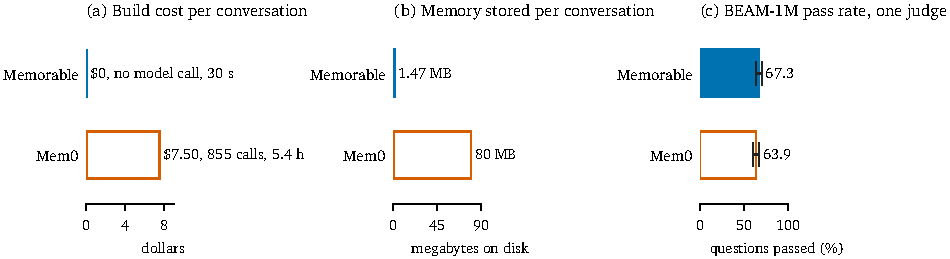
\includegraphics[width=\textwidth]{fig_lead3.pdf}
\caption{Build cost, bytes stored and pass rate for one 1M-token BEAM conversation. Left: model cost, calls and time to build the memory, measured on Mem0's open-source release over 80\% of the conversation and extrapolated to the whole. Middle: bytes stored on disk. Right: pass rate on BEAM-1M under one judge, 700 questions, with 95\% Wilson intervals. Per-question cost is in Figure~\ref{fig:breakeven}.}
\label{fig:lead}
\end{figure}

\begin{figure}[t]
\centering
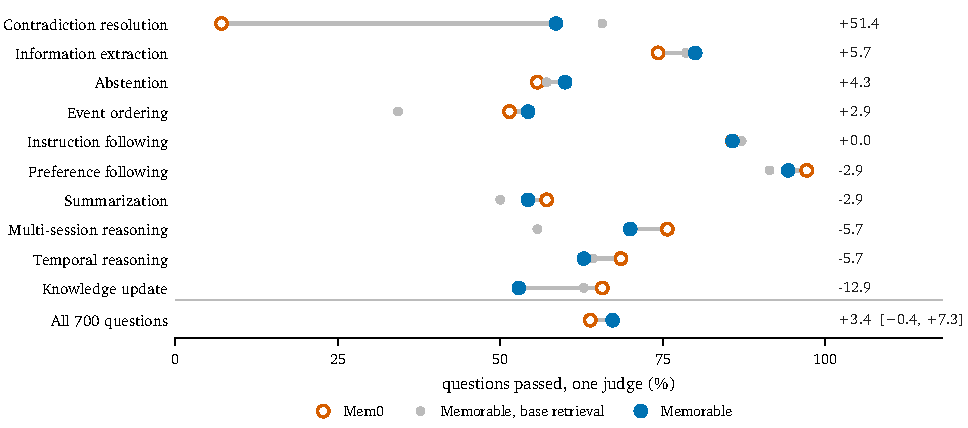
\includegraphics[width=\textwidth]{fig_abilities.pdf}
\caption{BEAM-1M by ability, one judge, 70 questions per ability. Hollow dots are Mem0, filled blue dots are Memorable and small grey dots are base retrieval. The grey line joins Mem0 to Memorable; the number at the right is Memorable minus Mem0 in points. The last row is all 700 questions with the bootstrap interval on the gap.}
\label{fig:abilities}
\end{figure}

\paragraph{Contradiction questions.} The largest gap between the two systems is here. These questions ask about a fact the user changed, and the rubric asks the answer to name both statements. In the first conversation the user writes ``I've completed the translation microservice and it's working great'' and, 158 turns later, that they have never completed it. Our reader sees both turns and says so: under the one judge the full method passes 58.6\% of these questions and base retrieval 65.7\%, against 7.1\% for Mem0. The gap holds under both judges that scored both systems, and its size varies with the judge. Mem0's own judge scores the same answers 48.6\% and BEAM's judge 15.7\%, and under BEAM's judge base retrieval scores 64.3\% and the full method 42.9\% (Appendix~\ref{app:ownjudge}). In Mem0's open-source release an UPDATE replaces the earlier fact, so the memory holds one version. Its hosted pipeline is closed, so we cannot confirm that the same step produced the 7.1\%.

\paragraph{What search adds.} Base retrieval trails Mem0 on the abilities whose evidence is spread over several sessions: multi-session reasoning by 20.0 points, event ordering by 17.1 and summarization by 7.1. One query finds one session, whereas a memory that a model wrote holds facts from every session in one store. The planner, the 60-turn read and the session cap are aimed at this gap. On the development sets (400 questions pooled over the 100K and 500K tiers, gpt-5-mini reader, BEAM's judge) they raise the pass rate from 74.2\% to 79.8\%, with multi-session reasoning moving from 67.5 to 82.5, event ordering from 52.5 to 70.0 and summarization from 65.0 to 80.0 (Figure~\ref{fig:ladder}). On the 1M tier under one judge the same components move multi-session reasoning from 55.7 to 70.0, event ordering from 34.3 to 54.3 and summarization from 50.0 to 54.3. They cost ground on two abilities: knowledge update falls from 62.9 to 52.9 and contradiction resolution from 65.7 to 58.6, and under BEAM's judge the contradiction drop is larger, 64.3 to 42.9. Of the 18 contradiction questions lost under that judge, half dropped a gold turn from the read set; in the other half the reader listed both statements as a dated timeline and left their conflict unnamed. The rubric requires the conflict to be named (Appendix~\ref{app:ownjudge}).

\paragraph{Where Mem0 stays ahead.} Mem0 leads on knowledge update by 12.8 points, and by 2.9 to 5.7 points, two to four questions of 70, on temporal reasoning, multi-session reasoning, preference following and summarization (Figure~\ref{fig:abilities}). Knowledge-update questions ask for the current value of a fact that changed. A memory that overwrites holds only that value, whereas our reader sees both turns and has to pick the later one; we did not test whether this explains the gap.

\begin{figure}[H]
\centering
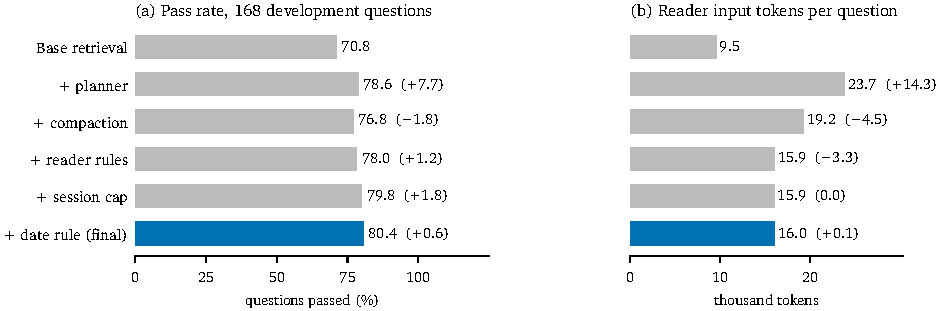
\includegraphics[width=\textwidth]{fig_ladder.pdf}
\caption{Adding the search components one at a time on the 500K development tier (development questions, separate from the 1M result): 168 questions every run answered, gpt-5-mini reader, BEAM's judge. Left: pass rate. Right: input tokens handed to the reader per question. The planner adds 7.7 points and 14.3K tokens; compaction and the reader rules return 7.8K of those tokens.}
\label{fig:ladder}
\end{figure}

\paragraph{The 10M tier.} Mem0 publishes answers for the ten conversations of BEAM's 10M-token tier, 200 questions, and we ran the full method on them once after registering predictions (Appendix~\ref{app:predictions}). Under the one judge Memorable passes 56.0\% and Mem0 46.5\%, a gap of 9.5 points with a registered interval of $[+0.5, +18.0]$ and a paired interval of $[+7.0, +12.0]$ (Figure~\ref{fig:abilities10m}). Memorable is ahead in each of the ten conversations, by one to three questions of 20; with all ten differences positive, a two-sided sign-flip test gives $p = 2/1024 = 0.002$. Contradiction resolution is 60.0\% against 10.0\% and temporal reasoning 50.0\% against 20.0\%, while Mem0 stays ahead on preference following, 90.0\% against 75.0\%, and on multi-session reasoning, 30.0\% against 25.0\%. Each ability has 20 questions here, so one question moves it by 5 points, and temporal reasoning changes sign between tiers (Mem0 ahead by 5.7 points on 1M, Memorable ahead by 30.0 here); we do not interpret that. The reader took 16,172 input tokens per question, and the run cost \$10.21, of which \$9.49 was the reader and the rest the planner and BEAM's judge in the run loop. The memory of a 10M-token conversation takes 16.7~MB, above the 10~MB we predicted.

\begin{figure}[H]
\centering
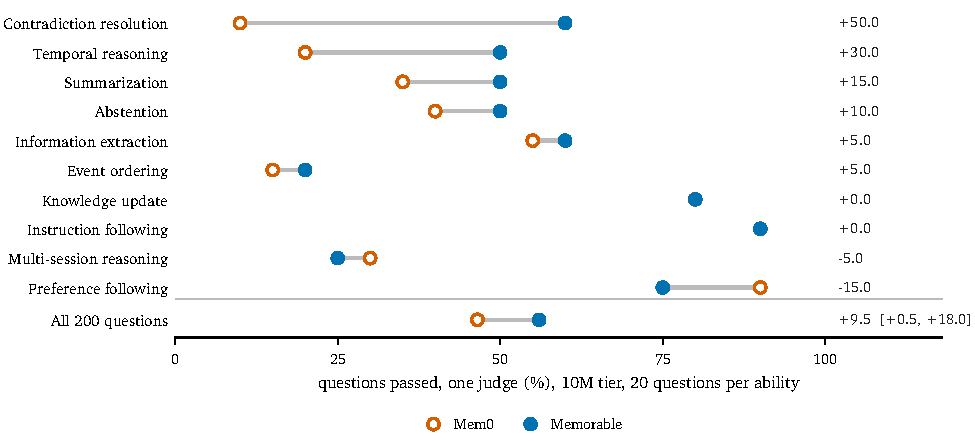
\includegraphics[width=\textwidth]{fig_abilities_10m.pdf}
\caption{BEAM-10M, 200 questions over ten conversations, one judge. Hollow orange: Mem0 (Platform v3, GPT-5). Filled blue: Memorable, full method with the 1M settings, run once. Right: the gap in points; the interval beside the All 200 questions row is the registered 95\% interval.}
\label{fig:abilities10m}
\end{figure}

\subsection{Cost and storage}
\label{sec:cost}

\paragraph{Build.} Building the memory of the first 1M conversation with Mem0's open-source release and gpt-5-mini as extractor took 683 extraction calls for 80\% of the turns before a \$6 cap stopped it: 6.85M input and 2.14M output tokens, 3,788 memory entries, 260 minutes at one worker and 64~MB on disk. Scaled to the whole conversation, that is about 855 calls, \$7.50, 5.4 hours and 80~MB (Table~\ref{tab:build}). Memorable builds the same conversation in about 30 seconds of CPU and stores 1.47~MB, 0.81~MB of compressed text and 0.66~MB of 8-bit vectors (Figure~\ref{fig:waterfall}). Mem0's facts take less text than our turns: about 4,700 entries for the whole conversation hold 1.15~MB against our 3.67~MB of compacted turns before compression, or 0.34~MB against 0.81~MB after zlib. Each entry also carries a float vector, 2.8 per turn and 7.3~MB in all, and the rest of the 80~MB is its vector database and index.

\begin{figure}[H]
\centering
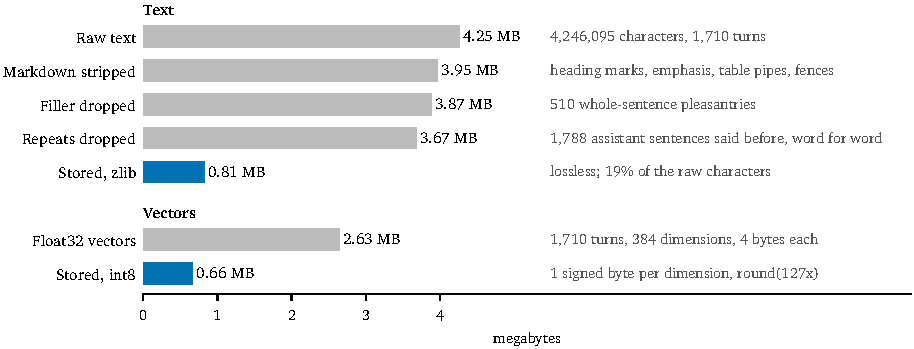
\includegraphics[width=\textwidth]{fig_waterfall.pdf}
\caption{Bytes kept at each step for the first 1M conversation. Text: raw, after each compaction rule, and after zlib. Vectors: float32 and 8-bit.}
\label{fig:waterfall}
\end{figure}

\paragraph{Per question.} Memorable's reader, GPT-5, takes 17,200 input tokens and produces 2,450 output tokens per question, \$0.046 at GPT-5 prices measured over the 700 questions, plus about \$0.001 for the planner call. Mem0's reader takes 200 facts of about 242 characters, about 12,100 input tokens, plus about 450 for the question and instructions. Mem0 publishes the facts and leaves out token counts, so we assume 1,500 output tokens; GPT-5 prices then give \$0.0307, which we write as \$0.031. With Equation~\ref{eq:cost} the two systems cost the same after about 460 questions on one conversation (Figure~\ref{fig:breakeven}).

\begin{figure}[H]
\centering
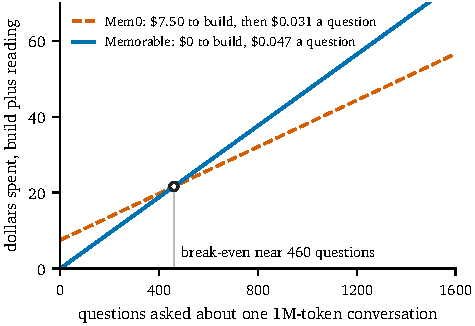
\includegraphics[width=0.55\textwidth]{fig_breakeven.pdf}
\caption{Dollars spent on one 1M-token conversation as questions accumulate. Mem0 starts at its measured build cost; Memorable starts at zero. Mem0's per-question cost is estimated from the size of its retrieved facts; ours is measured.}
\label{fig:breakeven}
\end{figure}

\subsection{LongMemEval-S}
\label{sec:lme}

\paragraph{Retrieval.} Keyword and embedding rankings fused by reciprocal rank and rescored by the cross-encoder place every gold session in the top 10 for 95.5\% of the 375 LongMemEval-S test questions with gold labels. EdgeMem reports 93.8\% and MemGAS 94.5\% \citep{cui2026edgemem,xu2025memgas}, and we read the published metrics as the same measure. The 95 development questions, on which we made the retrieval choices, score 92.6\%; all 470 together score 94.9\%. On LongMemEval-S most gold turns are the user's, so a rule that hands the reader every user turn in the top 60, and an assistant reply only when it ranks in the top 10, brings the input to 6,777 tokens and keeps every gold turn for 97.9\% of development questions. We have not run a reader on that setting.

\section{Related Work}
\label{sec:background}

We organize prior work by its stored representation: model-written summaries, facts or notes; verbatim interactions; and guidance derived from past agent runs. This separates the choice of what to store from the method used to retrieve it.

\paragraph{Model-written stores.}
MemoryBank and ReadAgent use a model to write summaries or gists of past sessions \citep{zhong2024memorybank,lee2024readagent}. Mem0 extracts candidate facts from each exchange with one model call and reconciles them against stored facts with another; its graph variant also extracts entities and relations \citep{chhikara2025mem0}. Zep builds a temporal knowledge graph with separate model passes for entities, facts, dates and contradictions \citep{rasmussen2025zep}. Supermemory and Hindsight also extract facts at ingest \citep{hindsight2025,supermemory2026longmembench}. Other systems give agents control over memory files or notes. MemGPT lets the agent move facts between its context window and an external store \citep{packer2023memgpt}, and Letta adds a background agent that rewrites memory files \citep{letta2025sleeptime}. A-MEM writes linked notes and revises earlier ones \citep{xu2025amem}, while MemGAS stores several granularities, including model-written summaries \citep{xu2025memgas}. These systems incur generative calls when constructing at least part of their memory representation.

\paragraph{Verbatim stores.}
EdgeMem and Chain-of-Memory are the closest comparisons to our approach because they retain turns and search them with local models. EdgeMem annotates verbatim turns with spaCy and searches two keyword indices, without generative model calls before the reader. It reports retrieval on LongMemEval-S \citep{cui2026edgemem}. Chain-of-Memory builds chains of turn embeddings using a large embedding model and, as far as its method section states, generates no text at build or search time \citep{xu2026com}. Our store adds an embedding search and two cross-encoder rerankers relative to EdgeMem, and a keyword search and two dialogue rules relative to Chain-of-Memory. Related retrieval work defers or simplifies graph construction, as in LazyGraphRAG and LinearRAG \citep{microsoft2024lazygraphrag,zhuang2025linearrag}. LongMemEval also shows that indexing at the right granularity recovers much of the gap between full context and an oracle history containing the answer evidence \citep{wu2025longmemeval}.

\paragraph{Procedural memories.}
These systems store information about how tasks were carried out. Agent Workflow Memory uses a model to induce workflows from past trajectories; its appendix also reports a rule-based variant scoring 35.6 on WebArena against 35.5 for the model-written variant \citep{wang2025agent}. Memp stores the raw trajectory, a model-distilled script, or both \citep{fang2026memp}. ReasoningBank uses a model to judge success and extract up to three items per trajectory \citep{ouyang2026reasoningbank}. ExpeL, Reflexion, Synapse, Voyager and SkillWeaver write insights, exemplars or executable skills with a model \citep{shinn2023reflexion,wang2024voyager,zhao2024expel,zheng2025skillweaver,zheng2024synapse}. We evaluate trajectory retrieval on Proced-Mem, which has 40 queries over a bank of agent trajectories, model-judged relevance and no held-out split \citep{procedmem}.

\paragraph{Benchmark and evaluation limits.}
LoCoMo has ten two-person conversations and 1,986 questions. Vendors score the 1,540 questions outside the adversarial category with the judge Mem0 introduced \citep{chhikara2025mem0,maharana2024locomo}. Two audits found 6.4 and 7.0 percent of its answer keys wrong, and one found that the judge accepted 62.81 percent of deliberately wrong on-topic answers \citep{coretoday2026audit,penfield2026locomoaudit}. Scores also depend on the reader and evaluation setup: full context scores 72.90 with gpt-4o-mini in Mem0's table and 92.85 with gpt-5-mini in a later study \citep{fullcontext2026}. Such cross-reader comparisons do not isolate the memory's contribution. LongMemEval has 500 questions over histories of about 115k tokens. Its September 2025 release replaced 454 histories, so results depend on which release is used \citep{coretoday2026audit,wu2025longmemeval}. BEAM has conversations of 128k to 10M tokens with 20 questions per conversation over ten abilities. Questions are graded item by item against rubric lists, but published rows do not always specify the judge model and prompt \citep{beam2026}. We use a shared reader and judge wherever a published per-question file permits it. Otherwise, we state the judges and treat differences as comparisons across evaluation setups rather than as a ranking of memories.

\section{Conclusion}
\label{sec:conclusion}

This paper asked whether a memory built by fixed code from the turns themselves can match one that a model writes. Memorable stores the conversation itself, compacted by fixed rules and compressed with zlib, and the first BEAM-1M conversation takes 1.47~MB; its model calls are the planner and the reader, both at question time. On BEAM-1M under one judge it passes 67.3\% of questions against Mem0's 63.9\%, a tie, since the interval on the gap includes zero; on the 10M tier it passes 56.0\% against 46.5\% and is ahead in each of the ten conversations. A memory that a model writes holds less text than the conversation, and it holds facts from every session in one store. That is where base retrieval trails. The planner and the two list rules close 14.3 of the 20.0-point gap on multi-session questions, from 55.7 to 70.0 against Mem0's 75.7. Keeping every turn is what lets the reader see both sides of a changed fact, and it is also what costs more tokens per question, so Mem0 is cheaper in total after about 460 questions on a conversation.

\paragraph{Limitations.} Several limitations must be acknowledged. (1) The judge is a model. We score both systems with one judge, but a different judge can still move an ability by tens of points: Mem0's contradiction answers score 48.6\% under its own judge, 15.7\% under BEAM's judge and 7.1\% under Claude Sonnet 5.5 (Appendix~\ref{app:ownjudge}). (2) Mem0's answers are from the file it published in March 2026; a fresh run of its hosted service might score differently, and we could not run it ourselves. (3) We tuned the full method on the 100K and 500K tiers and ran it once on 1M and once on the 10M questions Mem0 published, and the contradiction-resolution drop between base retrieval and the full method shows that a development set of 400 questions misses effects of this size. (4) Mem0's per-question read cost is estimated from the size of its retrieved facts; ours is metered. (5) On LongMemEval-S we measured retrieval alone, on the setting that fits Mem0's token budget. (6) Eight-bit vectors change the share of gold turns found by at most 0.4 points on the development set (Appendix~\ref{app:int8}). (7) On the first 1M conversation we inspected compaction's removals by frequency and found pleasantries and repeated closings; we have not read every removed sentence, so a lost fact would have escaped us. (8) The filler and repeat rules are written for English assistant prose and need new patterns for other languages or for agent tool logs. To address these, future work should score a fresh run of Mem0's hosted pipeline under the same judge, run a reader on the LongMemEval-S setting, and read every removed sentence.

\bibliographystyle{plainnat}
\renewcommand{\bibfont}{\small\raggedright}
\bibliography{refs}
\appendix
\section{Predictions}
\label{app:predictions}

Every run was registered before it started, with numbered predictions, and Table~\ref{tab:predictions} lists each one and whether it held. Ten missed: three scores landed above the registered range, five below it, one answer-model cost ran over its cap and one judge spread exceeded its bound. Eight registered on 2026-10-30 were never run, because the model budget ran out first; the one-judge re-scoring registered that evening ran once Anthropic credits arrived.

{\small
\begin{longtable}{@{}L{42mm}L{54mm}L{30mm}L{24mm}@{}}
\caption{Registered predictions. Held means the measured value fell inside the registered range or met the registered comparison.}\label{tab:predictions}\\
\toprule
Run & Prediction & Measured & Outcome \\
\midrule
\endfirsthead
\toprule
Run & Prediction & Measured & Outcome \\
\midrule
\endhead
\bottomrule
\endfoot
LoCoMo, BM25, 20 turns & 70 to 82 & 82.3 & missed by 0.3, high \\
BM25, 40 turns & at least 2 points over 20 turns & +3.5 & held \\
tuned retriever recall & all-gold recall at 20 turns at least 0.70 & 0.685 & missed \\
tuned retriever accuracy & at least 87 & 91.1 & held \\
full context & at least any retrieval pass; at least 10 times the cost & 95.7; 14 times & held \\
5r against 5a, Sonnet & at least 1.5 points & +1.8 & held \\
\midrule
adaptive cut, ranker with graph & test accuracy within 1.0 of 5r (94.9) & 94.8 & held \\
& mean turns read at most 16 & 12.9 & held \\
& second pass for at most 25 of 100 questions & 9.7 of 100 & held \\
& cost at or below 5r (\$10.80) & \$4.93 & held \\
adaptive cut, graph-free ranker & test accuracy within 1.0 of 94.8 & 94.5 & held \\
& mean turns within 1.0 of 12.9 & 13.2 & held \\
& all-gold recall at 10 on test within 1.5 of 74.7 & 72.7 & missed by 0.5 \\
\midrule
\lmes{}, 5a (registered for GPT-6 Sol, run with Sonnet) & 76 to 88 & 90.0 & missed, high \\
& above full context gpt-4o and Zep & 90.0 against 60.6 and 71.2 & held \\
& answer model under \$10 & \$13.23 & missed \\
\midrule
Proced-Mem, bge-m3 & 0.92 to 0.97 & 0.920 & held, at floor \\
& judge passes differ by under 0.02 & 0.024 & missed \\
\midrule
\multicolumn{4}{l}{\emph{Registered 2026-10-30 (Addenda 35, 36 and 39)}} \\
LoCoMo, v2 search, 150 turns, grouped dates, test & recall at 150 between 92 and 94.5, multi-hop 83 to 89 & 94.4; 86.1 & held \\
LoCoMo, v2 search, 40 turns, test & recall at 40 between 83 and 86 & 86.3 & missed by 0.3, high \\
LoCoMo, cascade rerank, test & recall at 40 within 0.5 of 86.3; at 150 within 0.5 of 94.4 & 86.1; 93.8 & held; missed by 0.1, low \\
LoCoMo, GPT-5, 40 turns, 933 test questions left & test accuracy 88 to 90.5 & -- & not run \\
LoCoMo, v2 search, 150 turns, grouped dates, GPT-5 reader & accuracy 90.0 to 92.5; multi-hop 85 to 91 & -- & not run \\
LoCoMo, Mem0's answers under the 2025 judge & 93.5 to 96.0 & -- & not run \\
\lmes{}, GPT-5, 100 turns, 81 test questions left & test 93 to 95 on 400 & -- & not run \\
\lmes{}, local reranker and user-turn rule, 60 turns & dev 92 to 95; test 93 to 95.5 & -- & not run \\
BEAM 1M, Mem0's answers under BEAM's judge & pass rate 62 to 72 & -- & not run \\
BEAM 1M, our answers under Mem0's judge & pass rate 66 to 76; ordering holds under both judges & -- & not run \\
LoCoMo and \lmes{}, Sonnet 5.5 reader, Mem0's prompts, GPT-5 judge & 150-turn LoCoMo arm 92 to 94.5 on test & -- & not run \\
\midrule
\multicolumn{4}{l}{\emph{Registered 2026-10-30, one judge for both systems (Addendum 41): Claude Sonnet 5.5 re-scores existing answers}} \\
LoCoMo, our 607 answers & 88 to 93; Mem0 within 2.0 on the same questions & 90.1; Mem0 90.0 & held \\
LoCoMo, Mem0's 1,540 answers & 89 to 93 & 91.3 & held \\
\lmes{}, both systems & ours 91 to 95; Mem0 91 to 95; gap under 2.5 & -- & not run: Mem0's file holds verdicts, not answers \\
BEAM 1M, both systems & ours 66 to 76; Mem0 64 to 74; gap under 4 & 61.3; 63.9; gap 2.6 & missed, low; missed, low; gap held \\
agreement of the one judge with the original judge on our answers & at least 90 percent on LoCoMo and \lmes{} & LoCoMo 99.0 and 98.6; \lmes{} 90.0 and 93.1 & held \\
\end{longtable}}

\section{Retrieval}
\label{app:retrieval}

The tables below give every retrieval system we ran on the frozen splits, so that the rows in the body can be checked against the baselines they beat, and the labels ``z 0.4'' and ``RRF'' name the fusion rule, z-score fusion at BM25 weight 0.4 or reciprocal rank fusion.

\begin{table}[H]
\centering
\small
\setlength{\tabcolsep}{2.6pt}
\begin{tabular}{lcccc}
\toprule
& A & \multicolumn{2}{c}{B} & \\
\cmidrule(lr){2-2}\cmidrule(lr){3-4}
System & @5 $\uparrow$ & @3 $\uparrow$ & @10 $\uparrow$ & Pooled $\uparrow$ \\
\midrule
BM25, official script & 75.5 & 69.8 & 84.0 & 76.4 \\
BM25, stemmed & 88.1 & 78.9 & 92.1 & 86.4 \\
MiniLM, max chunk & 86.4 & 76.1 & 94.6 & 85.7 \\
bge-base, max chunk & 93.4 & 83.1 & \textbf{97.9} & 91.4 \\
Contriever (re-impl.) & 92.1 & -- & -- & -- \\
EdgeMem-style (re-impl.) & 85.1 & 81.0 & 91.8 & 86.0 \\
Hybrid MiniLM, z 0.4 & 91.7 & 81.6 & 96.7 & 90.0 \\
Hybrid bge, RRF & 93.0 & 81.9 & 96.1 & 90.3 \\
Flat fusion (bge, z 0.4) & \underline{95.0} & \underline{84.3} & 96.7 & 92.0 \\
\midrule
Ours & \textbf{95.4} & \underline{84.3} & 97.3 & \underline{92.3} \\
Ours + MiniLM rerank & \underline{95.0} & \textbf{87.3} & \underline{97.6} & \textbf{93.3} \\
\bottomrule
\end{tabular}
\caption{All systems we ran on the \lmes{} test split, session level, \rall{k}. Track A has $n{=}302$ and scores user turns against the official gold labels. Track B has $n{=}331$. Pooled is the mean of the three columns. Here and in Table~\ref{tab:locomoret}, the best value in each column is bold and the second best underlined.}
\label{tab:lmeall}
\end{table}

\begin{table}[H]
\centering
\small
\setlength{\tabcolsep}{4pt}
\begin{tabular}{lcccc}
\toprule
& \multicolumn{3}{c}{A} & B \\
\cmidrule(lr){2-4}\cmidrule(lr){5-5}
System & @5 $\uparrow$ & @10 $\uparrow$ & @50 $\uparrow$ & @10 $\uparrow$ \\
\midrule
BM25, official script & 50.0 & 59.9 & 77.5 & 54.4 \\
BM25, stemmed & 64.9 & 75.2 & 91.1 & 70.7 \\
bge-base, max chunk & 71.9 & 83.8 & 97.7 & 74.0 \\
Contriever (re-impl.) & 66.9 & 83.1 & 96.7 & -- \\
EdgeMem-style (re-impl.) & 62.6 & 73.2 & 94.7 & 61.0 \\
Flat fusion (bge, z 0.4) & \textbf{72.8} & \textbf{87.1} & \textbf{99.0} & \textbf{80.1} \\
\bottomrule
\end{tabular}
\caption{\lmes{} turn-level \rall{k} on the test split, Track A $n{=}302$ and Track B $n{=}331$. No published row exists for turn level on S. The flat fusion is the frozen turn-level system; on development it scored 74.4, 83.8 and 97.4 on Track A, and no turn-level variant scored above it.}
\label{tab:lmeturn}
\end{table}

\begin{table}[H]
\caption{\lmes{} retrieval on the frozen split, test questions read once. The test split has 400 questions, and 375 are scored after dropping abstention questions. Session metrics are derived from the turn ranking. R$_{\mathrm{any}}$ counts a question when at least one gold item is in the top $k$; R$_{\mathrm{all}}$ when every gold item is. 5r was picked on the 95 scored development questions by turn-level R$_{\mathrm{all}}$@5.}
\label{tab:lme-retrieval}
\scriptsize
\setlength{\tabcolsep}{2pt}
\centering
{\begin{tabular}{@{}lccccc|ccccc@{}}
\toprule
& \multicolumn{5}{c|}{session level} & \multicolumn{5}{c}{turn level} \\
Retriever & R$_{\mathrm{any}}$@5 & R$_{\mathrm{all}}$@5 & R$_{\mathrm{any}}$@10 & R$_{\mathrm{all}}$@10 & NDCG@10 & R$_{\mathrm{any}}$@5 & R$_{\mathrm{all}}$@5 & R$_{\mathrm{any}}$@10 & R$_{\mathrm{all}}$@10 & NDCG@10 \\
\midrule
BM25 (bm25s) & 84.0 & 68.3 & 90.4 & 76.5 & 65.6 & 78.4 & 55.2 & 85.6 & 68.8 & 64.1 \\
bge-small, dense & 92.3 & 76.3 & 95.7 & 89.3 & 64.9 & 81.9 & 53.3 & 90.1 & 72.3 & 61.9 \\
z-score fusion, 0.4 BM25 + 0.6 dense & 93.6 & 80.0 & 97.9 & 89.9 & 73.2 & 86.9 & 63.2 & 92.8 & 78.7 & 71.0 \\
5a, RRF & 95.5 & 81.6 & 97.9 & 92.3 & 72.2 & 87.7 & 61.1 & 94.7 & 80.5 & 70.5 \\
5r, 5a + reranker & \ours{97.6} & \ours{87.2} & \ours{99.2} & \ours{95.5} & \ours{80.9} & \ours{93.1} & \ours{73.6} & \ours{96.0} & \ours{85.1} & \ours{79.1} \\
\bottomrule
\end{tabular}}
\end{table}

\begin{table}[H]
\caption{LoCoMo retrieval on the frozen split. Development: conversations 26, 30 and 41 (383 questions). Test: the other seven (1,153), read once. The pick rule, fixed first, was R$_{\mathrm{all}}$@5 on development, which 5r won.}
\label{tab:locomo-retrieval}
\small
\begin{tabular}{@{}lcc|cccc@{}}
\toprule
& \multicolumn{2}{c|}{development} & \multicolumn{4}{c}{test} \\
Retriever & Hit@1 & R$_{\mathrm{all}}$@5 & Hit@1 & R$_{\mathrm{all}}$@5 & R$_{\mathrm{all}}$@10 & R$_{\mathrm{all}}$@40 \\
\midrule
BM25 & 0.329 & 0.493 & 0.337 & 0.469 & 0.532 & 0.645 \\
cleaned, stemmed BM25 & 0.397 & 0.517 & -- & -- & -- & -- \\
bge-small, dense & 0.295 & 0.488 & -- & -- & -- & -- \\
5a, RRF & 0.373 & 0.530 & -- & -- & -- & -- \\
z-score fusion, best weight 0.4 & 0.420 & 0.574 & -- & -- & -- & -- \\
5r, 5a + reranker & \ours{0.470} & \ours{0.616} & \ours{0.474} & \ours{0.595} & \ours{0.668} & \ours{0.781} \\
\bottomrule
\end{tabular}
\end{table}

\begin{table}[H]
\centering
\small
\begin{tabular}{lcccccccc}
\toprule
& \multicolumn{4}{c}{Text only} & \multicolumn{4}{c}{Text plus image caption} \\
\cmidrule(lr){2-5}\cmidrule(lr){6-9}
System & @5 $\uparrow$ & @10 $\uparrow$ & @25 $\uparrow$ & @50 $\uparrow$ & @5 $\uparrow$ & @10 $\uparrow$ & @25 $\uparrow$ & @50 $\uparrow$ \\
\midrule
BM25, official script & 29.7 & 36.6 & 46.9 & 53.6 & 28.9 & 37.0 & 47.3 & 55.2 \\
BM25, stemmed & 45.9 & 54.8 & 63.9 & 70.7 & 45.6 & 54.2 & 64.8 & 71.3 \\
bge-base, max chunk & 46.7 & 55.8 & 69.4 & 79.8 & 44.3 & 53.1 & 67.5 & 77.9 \\
EdgeMem-style (re-impl.) & 50.2 & 62.9 & 74.5 & 79.2 & 49.3 & 62.4 & 74.7 & 79.7 \\
Flat fusion (bge, z 0.4) & 55.0 & 64.0 & 73.9 & 80.9 & 53.9 & 63.5 & 74.2 & 81.4 \\
\quad + forward contiguity & 59.4 & 68.5 & 77.6 & 83.5 & 58.1 & 67.7 & 77.4 & 84.0 \\
Ranker with graph, no cross-encoders & 67.5 & 75.4 & 84.1 & \underline{88.9} & 66.6 & 74.8 & 84.4 & \underline{89.2} \\
First-round chain & 70.9 & 77.6 & \underline{85.0} & \underline{88.9} & 70.7 & 77.4 & 85.3 & \underline{89.2} \\
Graph-free ranker & \underline{74.0} & \underline{80.3} & \underline{85.0} & 88.5 & \underline{74.9} & \underline{79.7} & \underline{85.6} & 88.7 \\
\midrule
Ranker with graph & \textbf{75.9} & \textbf{81.5} & \textbf{86.8} & \textbf{90.1} & \textbf{75.8} & \textbf{81.4} & \textbf{87.0} & \textbf{90.3} \\
\bottomrule
\end{tabular}
\caption{Turn retrieval on LoCoMo test conversations 3 to 9 (1,152 questions): mean share of gold turns in the first $k$. The ranker with graph is the frozen configuration with the entity graph, the entity field and backward contiguity. The graph-free ranker is the store of Section~\ref{sec:turns}. The first-round chain reranks the top 50 turns with MiniLM alone. The other two rerank the top 100 with both cross-encoders. All rows are our own runs through one scorer. No published row is measured the same way.}
\label{tab:locomoret}
\end{table}

\begin{table}[H]
\centering
\small
\setlength{\tabcolsep}{2.5pt}
\begin{tabular}{llr}
\toprule
Change & Metric & $\Delta$ \\
\midrule
\multicolumn{3}{l}{\emph{\lmes{} development}} \\
Contiguity, turn level & A turn@5 & $-$16.2 [$-$23.9, $-$9.4] \\
PPR at weight 0.1 & pooled & $-$0.05 [$-$1.06, +0.96] \\
Entity, fact, date terms & pooled & 0 to $-$0.81 \\
\midrule
\multicolumn{3}{l}{\emph{LoCoMo development, flat fusion}} \\
BM25 weight 0.4 to 0.25 & recall@10 & +2.1 [$-$0.3, +4.4] \\
\midrule
\multicolumn{3}{l}{\emph{LoCoMo development, removed from the ranker with graph}} \\
Both cross-encoders & recall@10 & $-$6.8 \\
Contiguity (fwd., bwd.) & recall@10 & $-$1.9 \\
Speaker prior & recall@10 & $-$0.9 \\
PPR, entity field, bwd. & recall@10 & $-$0.7 \\
MiniLM cross-encoder & recall@10 & $-$0.4 \\
PPR alone & recall@10 & +0.1 \\
\bottomrule
\end{tabular}
\caption{Experiments run on development only. \lmes{} rows change the system named in each row; pooled is the development objective, the mean of Track A \rall{5} and Track B \rall{3} and \rall{10}. The last block removes components from the frozen LoCoMo system on the three development conversations; with three clusters we give no intervals. PPR is personalized PageRank.}
\label{tab:dev}
\end{table}

On the LoCoMo test conversations, recall of every gold turn at 5 by category moves from 0.038 to 0.135 on multi-hop, 0.528 to 0.654 on temporal, 0.164 to 0.274 on open-domain and 0.622 to 0.760 on single-hop, between BM25 and the ranker with the two cross-encoders, and multi-hop is the lowest category.

\section{Costs}
\label{app:costs}

Every dollar spent in this paper went to a reader or a judge, since building the store makes no generative write call, and Table~\ref{tab:costs} gives each answer run's cost at list prices.

\begin{table}[H]
\caption{Token-priced cost of each answer run, at list prices. Judge tokens are not included, except in the last row, which is a judge-only run.}
\label{tab:costs}
\footnotesize
\setlength{\tabcolsep}{3pt}
\begin{tabular}{@{}L{40mm}lr@{}}
\toprule
Run & Model & Cost \\
\midrule
LoCoMo, BM25 20 turns, 1,540 questions & GPT-6 Sol & \$4.16 \\
LoCoMo, BM25 40 turns & GPT-6 Sol & \$7.63 \\
LoCoMo, 5a & GPT-6 Sol & \$7.42 \\
LoCoMo, whole conversation in the prompt & GPT-6 Sol & \$105.81 \\
LoCoMo, 5a & Sonnet 5.5 & \$10.51 \\
LoCoMo, 5r & Sonnet 5.5 & \$10.80 \\
\lmes{}, 5a, 500 questions & Sonnet 5.5 & \$13.23 \\
Proced-Mem, three judge passes & gpt-5 judge & about \$2 \\
LoCoMo, BEAM and \lmes{} answers of both systems re-judged by one judge & Claude Sonnet 5.5 & about \$49, from token counts \\
\bottomrule
\end{tabular}
\end{table}


\end{document}
